
%	Presentacion de la comunidad linux uni
%	¿Que es GNU/Linux? - Escogiedo la libretad
%	search.sam@ - 20120617


\documentclass[xcolor=svgnames]{beamer}

\usepackage[spanish]{babel}
\usepackage[T1]{fontenc}
\usefonttheme{professionalfonts}
\usecolortheme{dolphin}

\mode<presentation>{\usetheme{default}}
%\usecolortheme[RGB={255,255,255}]{structure}
\setbeamertemplate{background}{
\includegraphics[width=\paperwidth]{fondo.png}}

% pre'ambulo
\author{\textbf{Samuel J. Guti\'errez Avil\'es} \\ \href{search.sam@gmail.com}{search.sam@gmail.com}}
\institute{\href{http://clinux.uni.edu.ni/}{Comunidad Linux Uni} \\ Comunidad de GNU/Linux de la Universidad Nacional de Ingenieria}
\date{20 de Junio, 2012}
\title{\textbf{Qu\'e es GNU/Linux?}}
\subtitle{Escogiendo la libertad!}

% cuerpo del documento
\begin{document}

	\begin{frame}
	
		\titlepage
		
	\end{frame}
	
%%%%%%%%%%%%%%%%%%%%%%%%%%%%%% slide - 1.

	\begin{frame}
	
		\frametitle{\textbf{Contenido de esta Presentaci\'on}}
		
			\begin{itemize}
				\item Linux
				\item Usos
				\item Repositorios
				\item Configuracion
			\end{itemize}

	\end{frame}

%%%%%%%%%%%%%%%%%%%%%%%%%%%%%% slide - 2.
%
%	\begin{frame}
%	
%		\frametitle{\textbf{Linux}}
%						
%			\begin{itemize}
%				\item Sistema Operativo
%				\item Software Libre
%				\item Distribucion 
%			\end{itemize}
%
%	\end{frame}
%
%%%%%%%%%%%%%%%%%%%%%%%%%%%%%% slide - 3.

	\begin{frame}
	
		\frametitle{\textbf{Linux:}:[Sistema Operativo]}
		
			\begin{wrapfigure}{r}{40mm}
				\begin{center}
					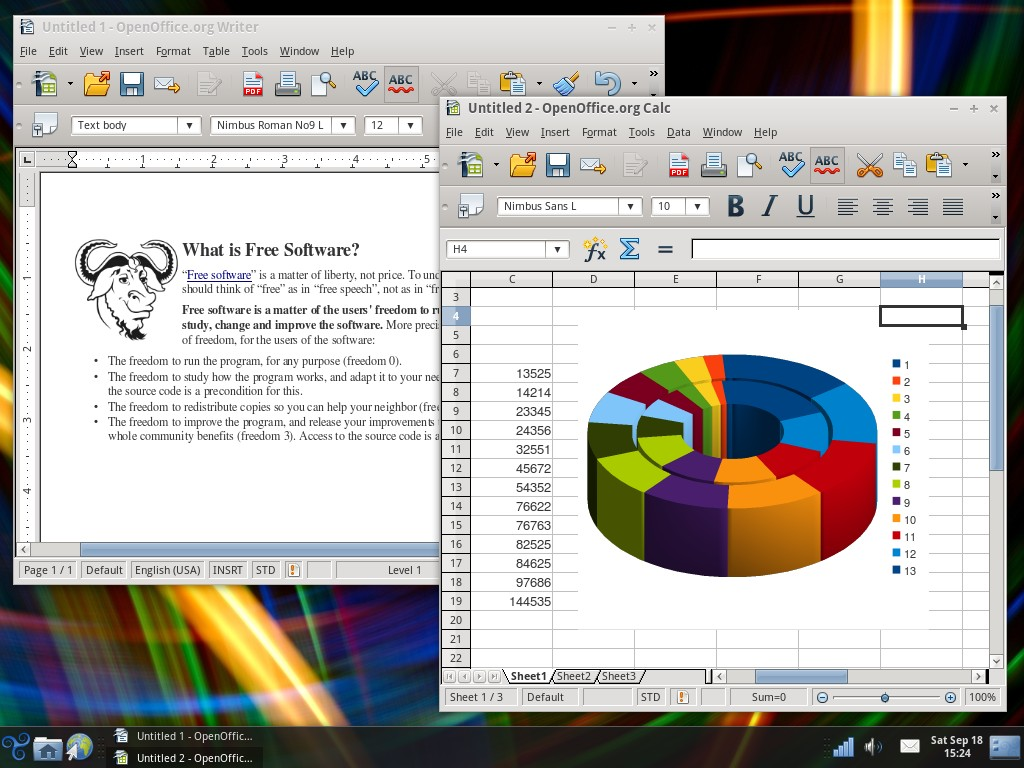
\includegraphics[height=0.35\textheight]{desktop.jpg}
				\end{center}
				\caption{Escritorio Linux}
			\end{wrapfigure}
			
			GNU/Linux es un sistema operativo similar a Unix que es software libre y respeta su libertad. Puede instalar versiones de GNU basadas en Linux que son completamente software libre. \\
			
			GNU/Linux es que se trata de un sistema operativo:
			\begin{itemize}
				\item Multiplataforma
				\item Multitarea
				\item Multiusuario
				\item Adaptable
			\end{itemize}

	\end{frame}
	
	%%%%%%%%%%%%%%%%%%%%%%%%%%%%%% slide - 4.

	\begin{frame}
	
		\frametitle{\textbf{Linux:}:[Software Libre]}
		
			\begin{wrapfigure}{r}{40mm}
				\begin{center}
					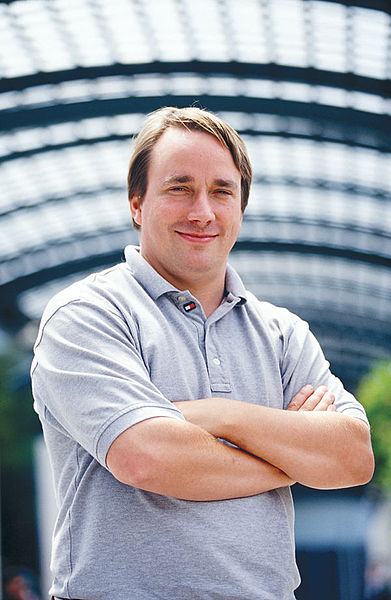
\includegraphics[height=0.45\textheight]{torvalds.jpeg}
				\end{center}
				\caption{Linus Torvalds}
			\end{wrapfigure}
			
			Sistema en s\'i no cuesta dinero y, a diferencia de Windows, el CD-ROM completo puede copiarse, prestarse o instalarse en varias m\'aquinas sin violar ninguna ley y con el benepl\'acito de sus autores.
			
			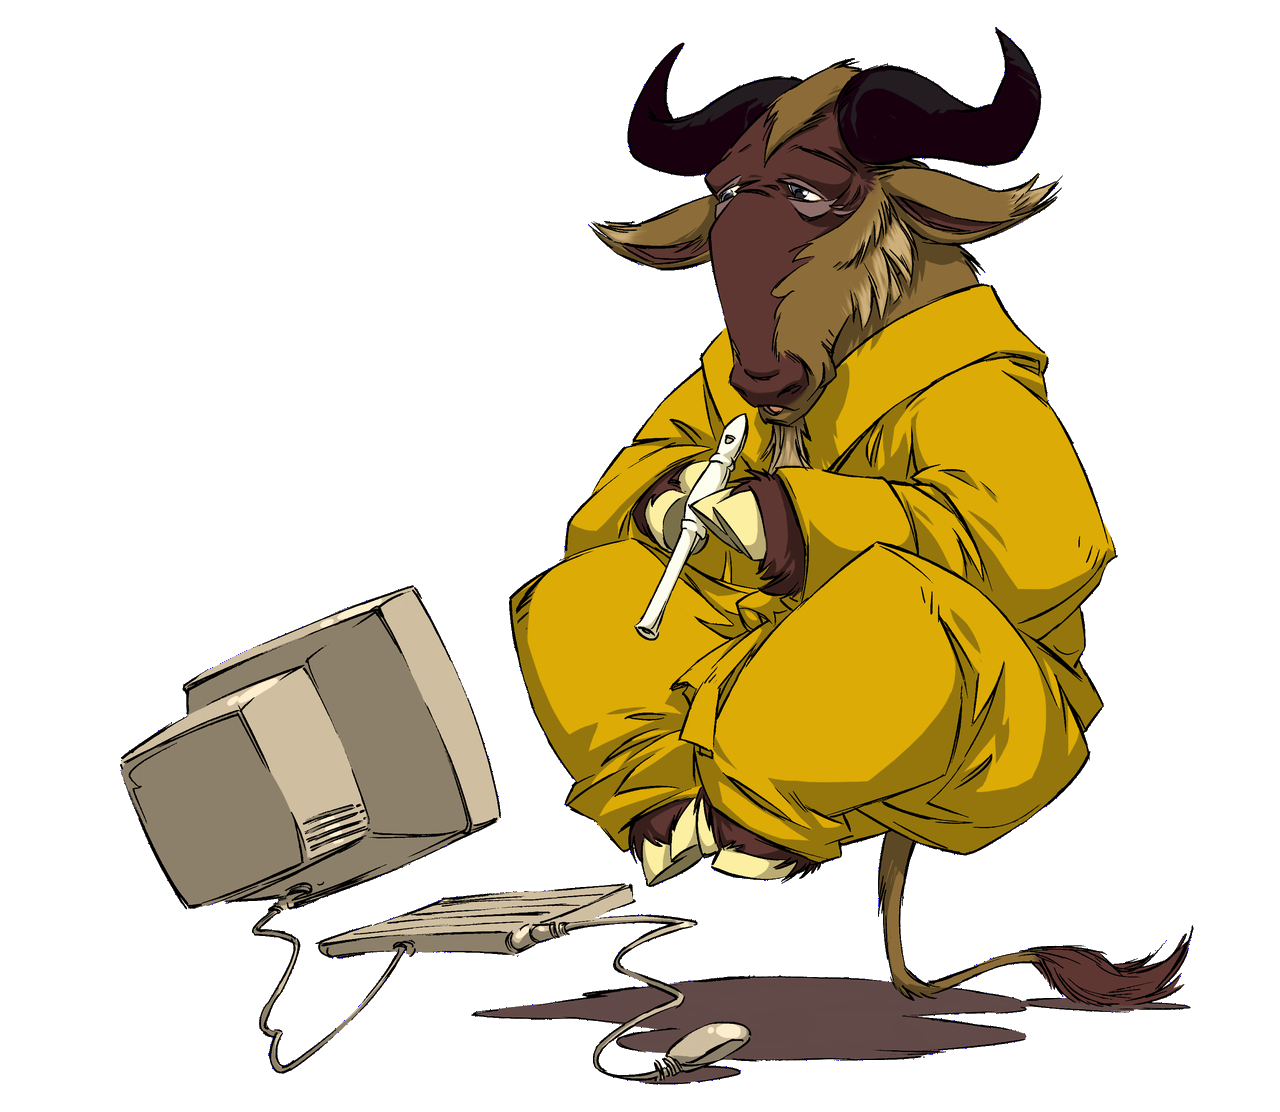
\includegraphics[height=0.45\textheight]{meditate.png}
			
	\end{frame}

%%%%%%%%%%%%%%%%%%%%%%%%%%%%%% slide - 5.

	\begin{frame}
	
		\frametitle{\textbf{Linux:}:[Distribuci\'on]}
		
			No es mas que una compilaci\'on de software como podr\'ian ser aplicaciones mas el n\'ucleo de Linux o sistema compilado listo para ser instalado para su posterior funcionamiento. 
			
			\begin{center}
				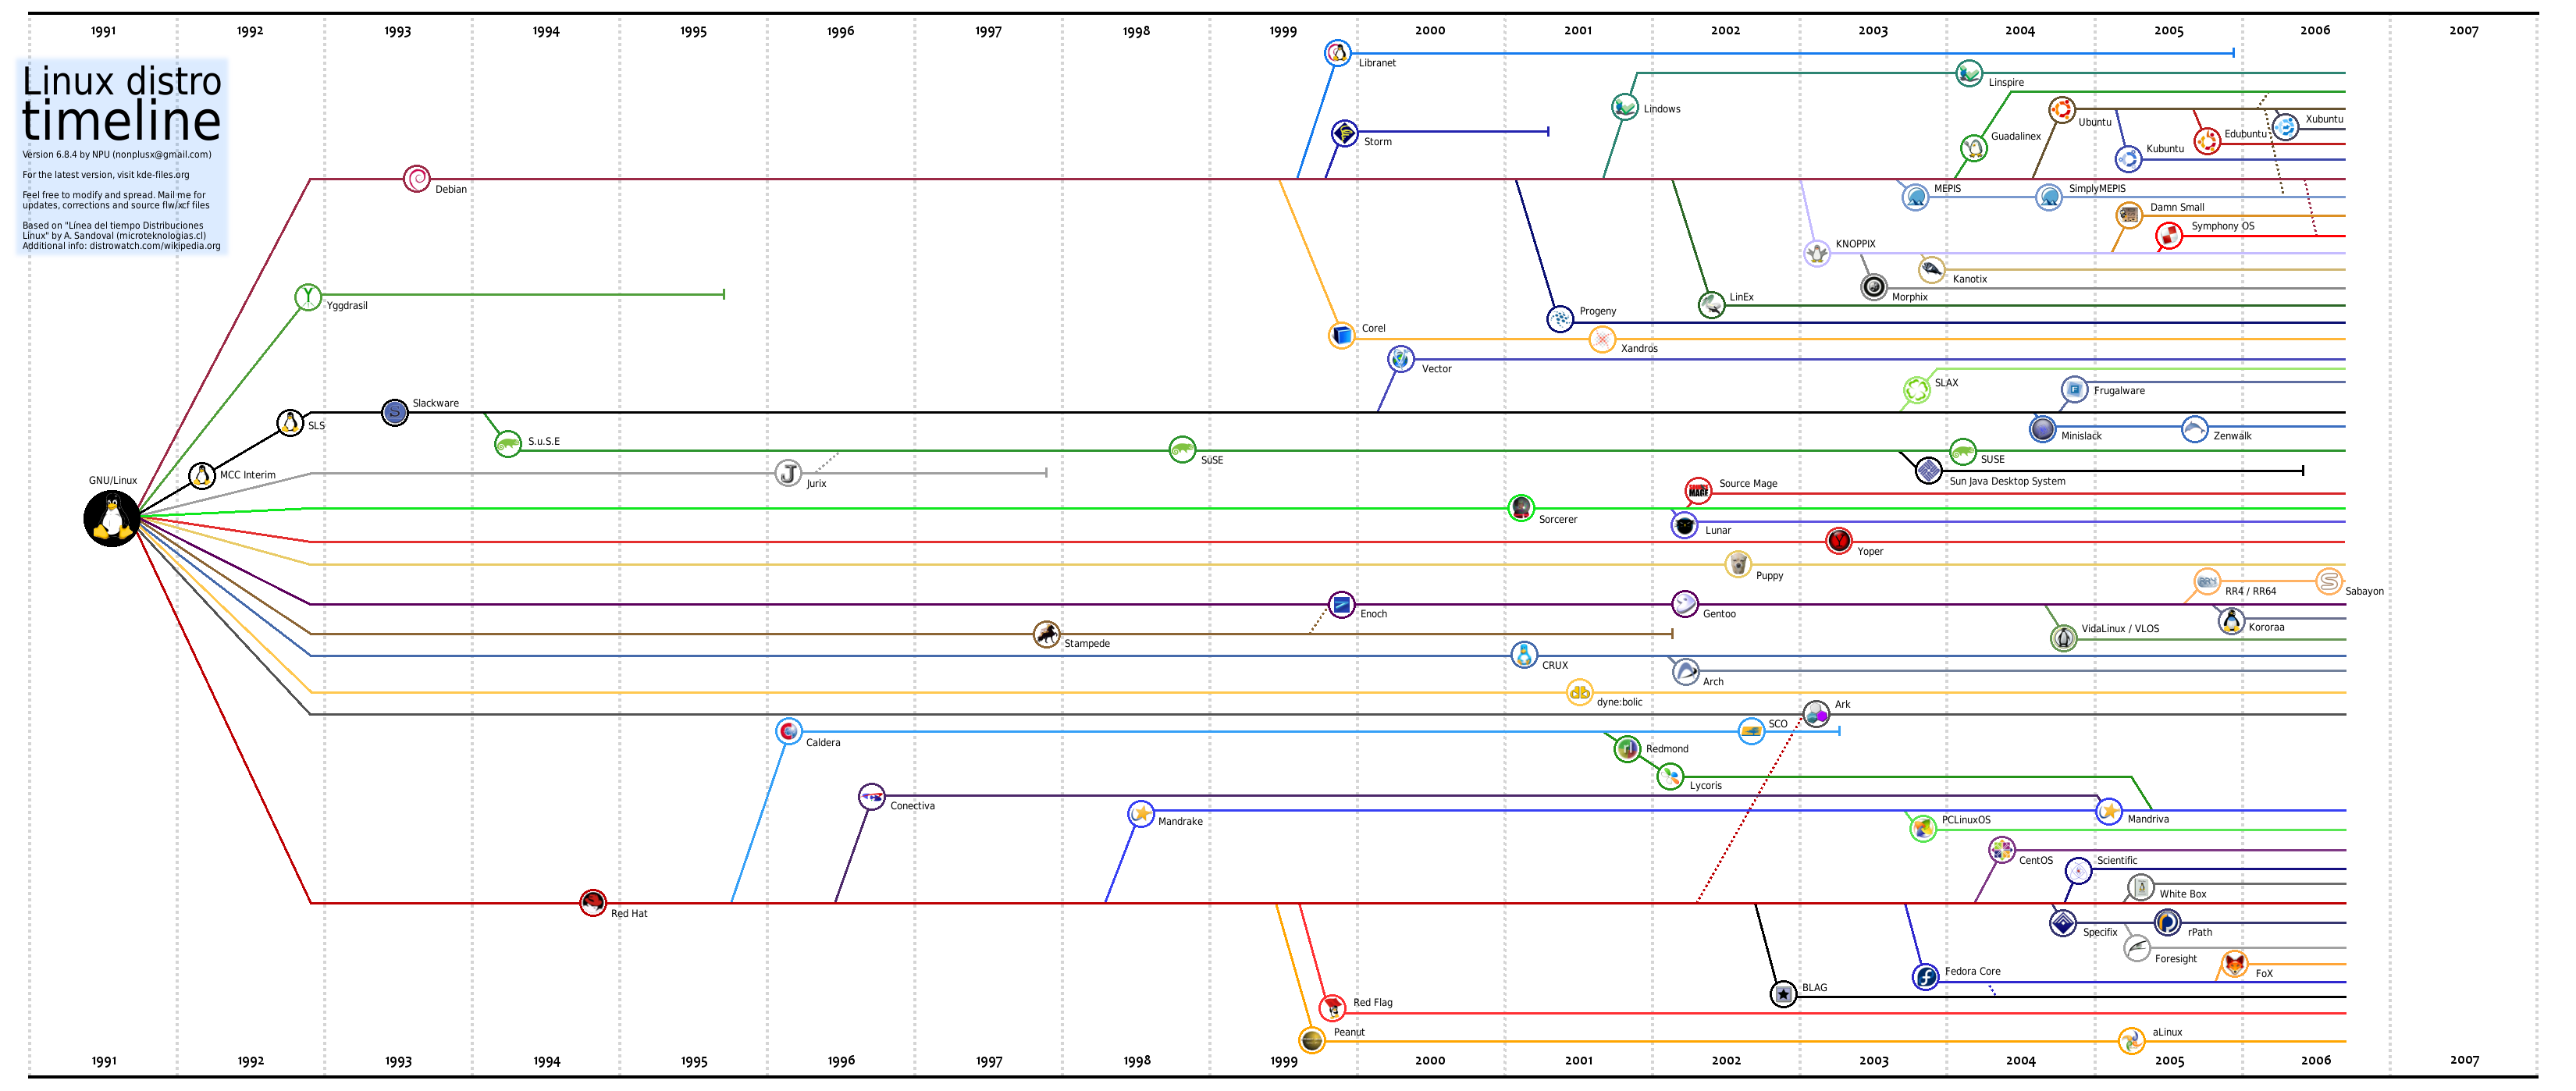
\includegraphics[height=0.45\textheight]{timeline.png}
			\end{center}
			
	\end{frame}

%%%%%%%%%%%%%%%%%%%%%%%%%%%%%% slide - 5.

	\begin{frame}
	
		\frametitle{\textbf{Linux:}:[...Distribuci\'on]}
		
			\begin{columns}
			
				\column{0.5\textwidth}
					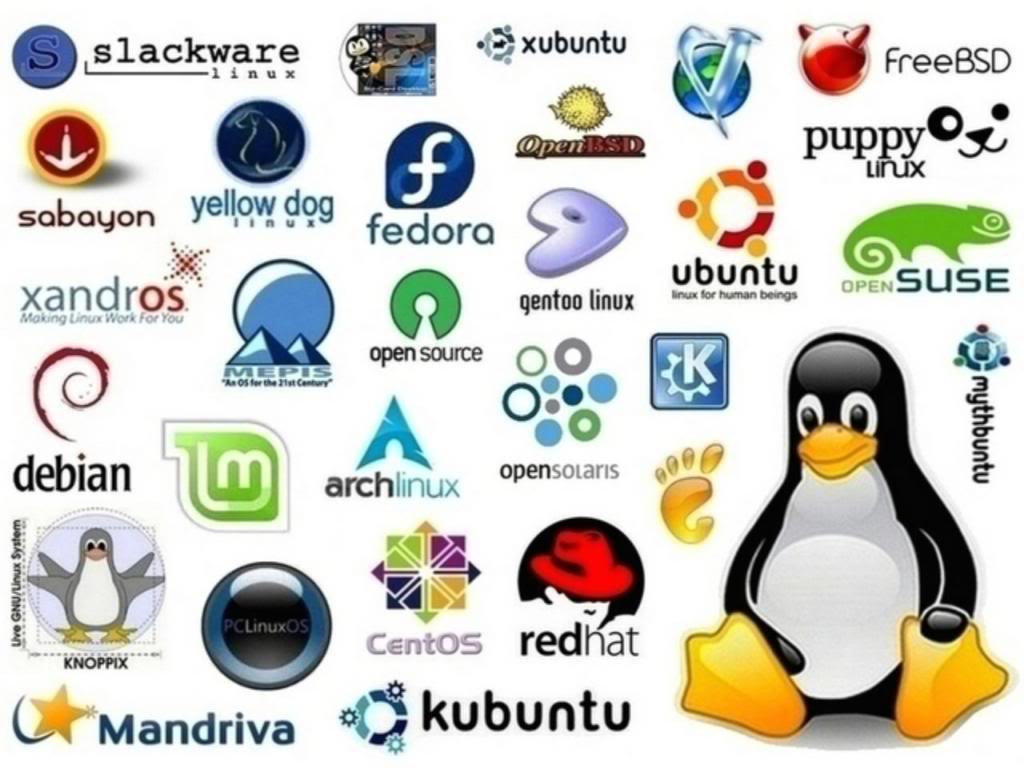
\includegraphics[height=0.35\textheight]{universe.jpg}

				\column{0.5\textwidth}
					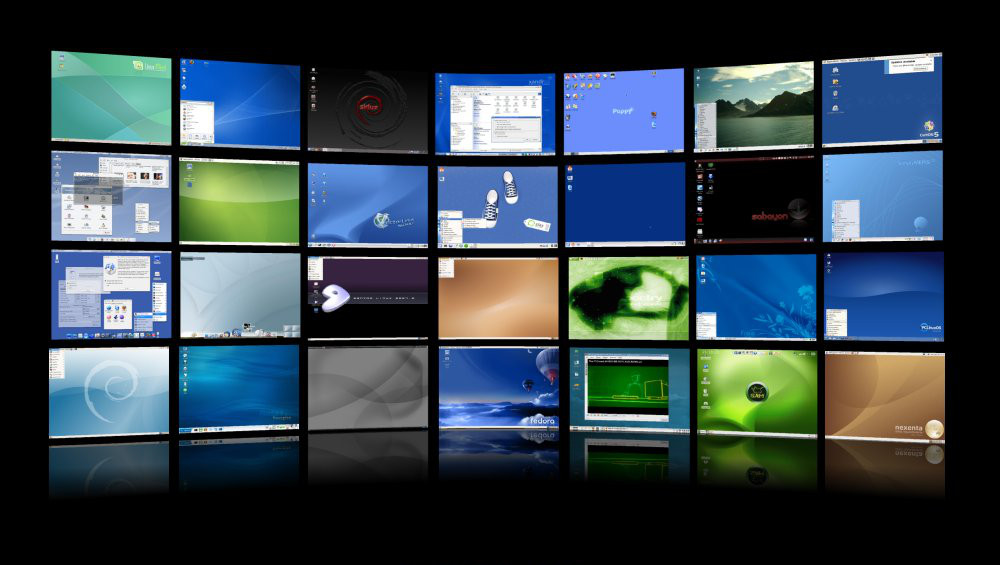
\includegraphics[height=0.35\textheight]{distros.jpg}
					
			\end{columns}
			
			\begin{center}
				
\includegraphics[height=0.35\textheight]{linux-logo.png} 
			\end{center}
			
	\end{frame}

%%%%%%%%%%%%%%%%%%%%%%%%%%%%%% slide - 6.
%
%	\begin{frame}
%	
%		\frametitle{\textbf{Usos}}
%						
%			\begin{itemize}
%				\item Uso general
%				\item Servicio dedicado
%				\item Ingenieria
%			\end{itemize}
%
%	\end{frame}
%	
%%%%%%%%%%%%%%%%%%%%%%%%%%%%%% slide - 7.

	\begin{frame}
	
		\frametitle{\textbf{Usos:}:[Aplicaci\'ones]}
		
		\begin{columns}
			
				\column{0.2\textwidth}{Cotidiano}
					\begin{center}
						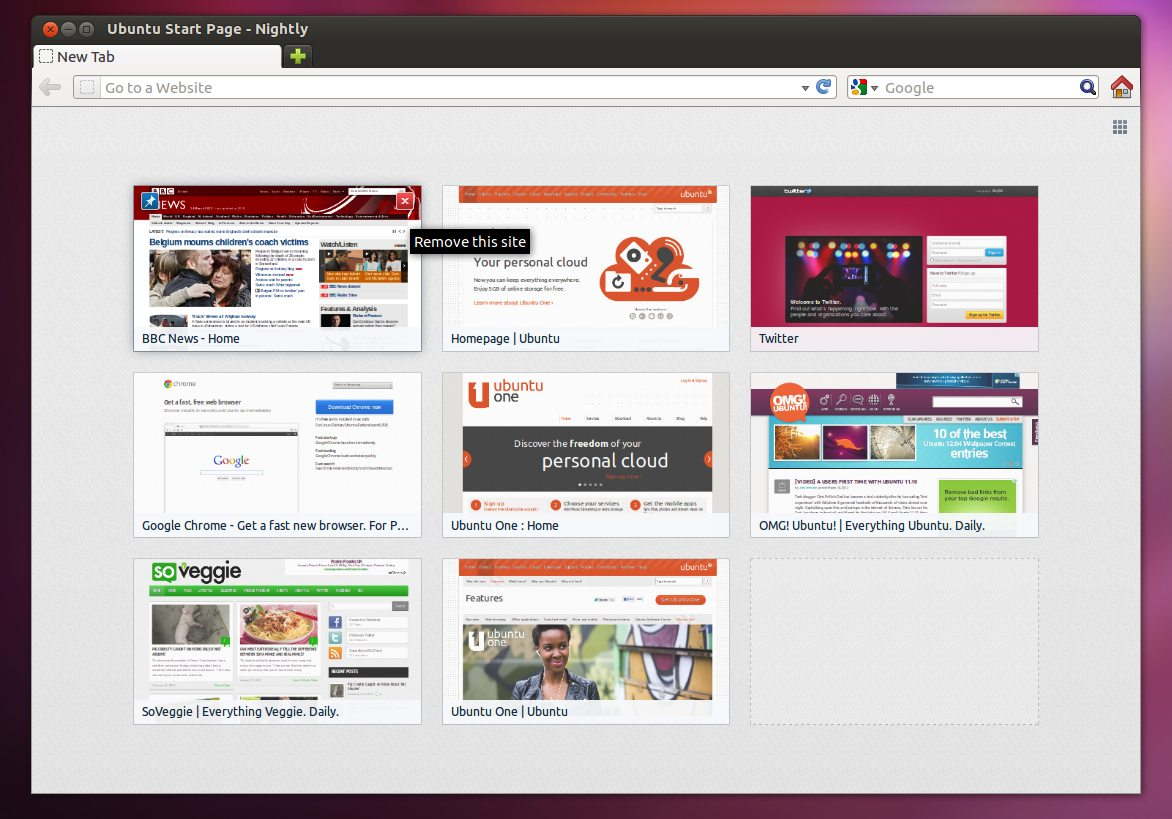
\includegraphics[height=0.20\textheight]{firefox.jpg} \\
						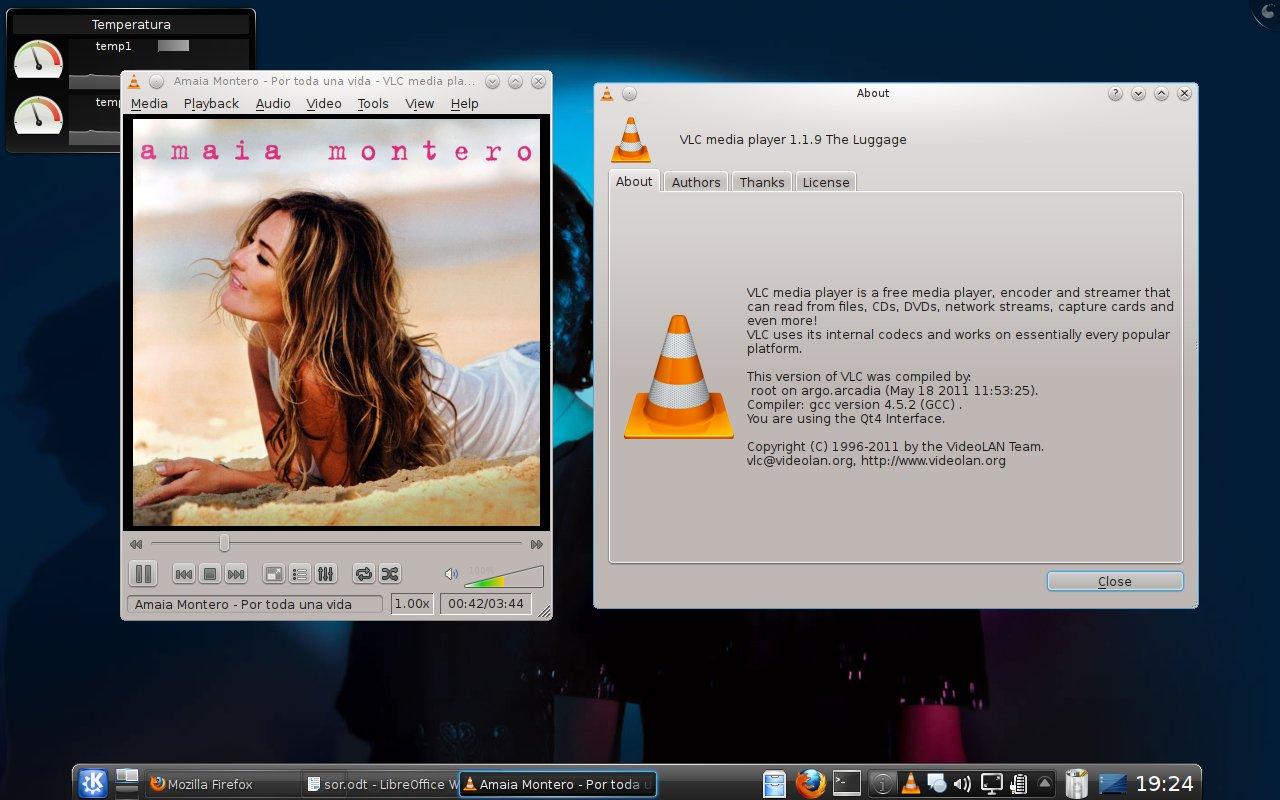
\includegraphics[height=0.20\textheight]{vlc.jpeg} \\
						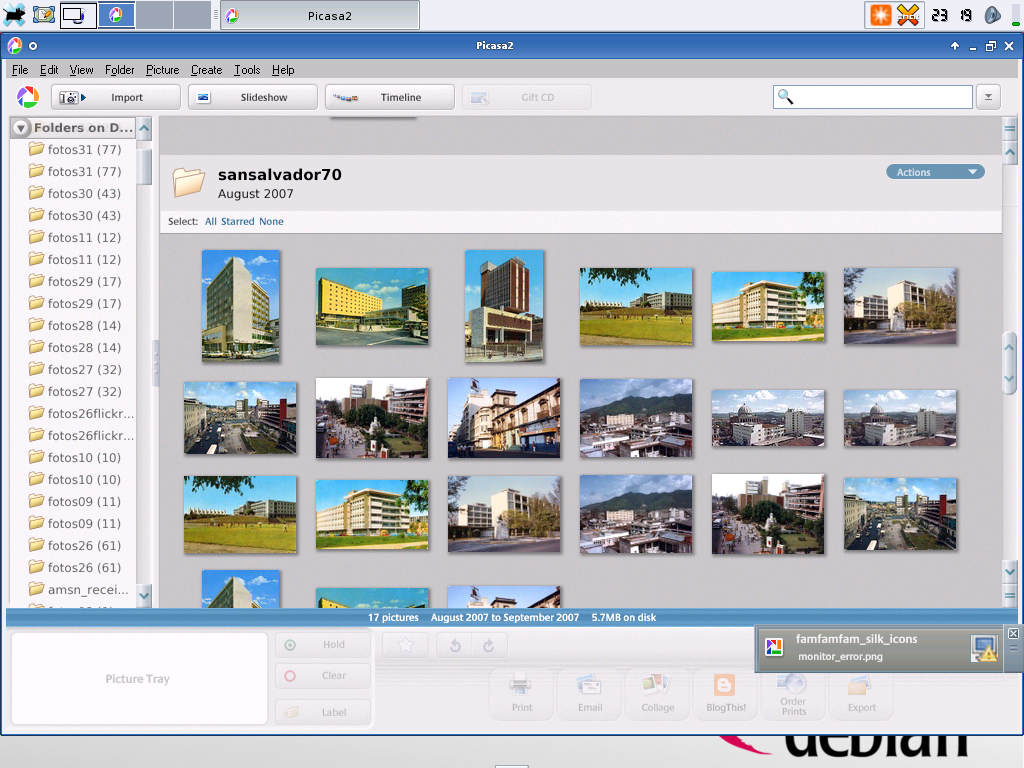
\includegraphics[height=0.20\textheight]{picasa.png}
					\end{center}

				\column{0.2\textwidth}{Servicio Dedicado}
					\begin{center}					
						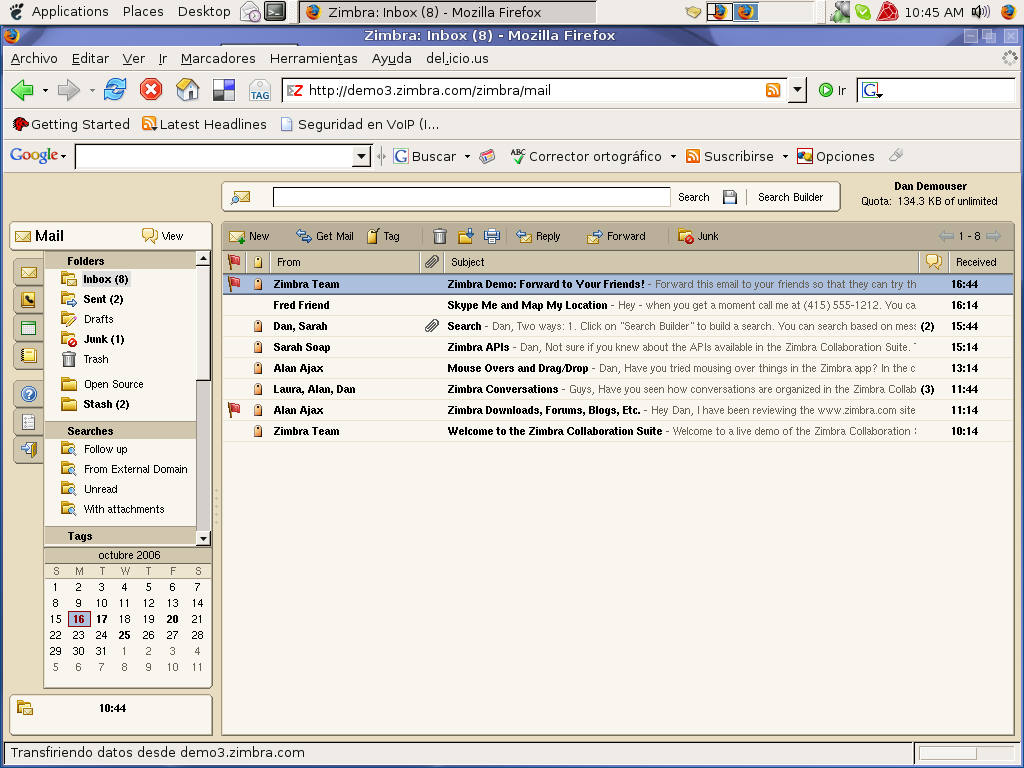
\includegraphics[height=0.20\textheight]{zimbra.png} \\
						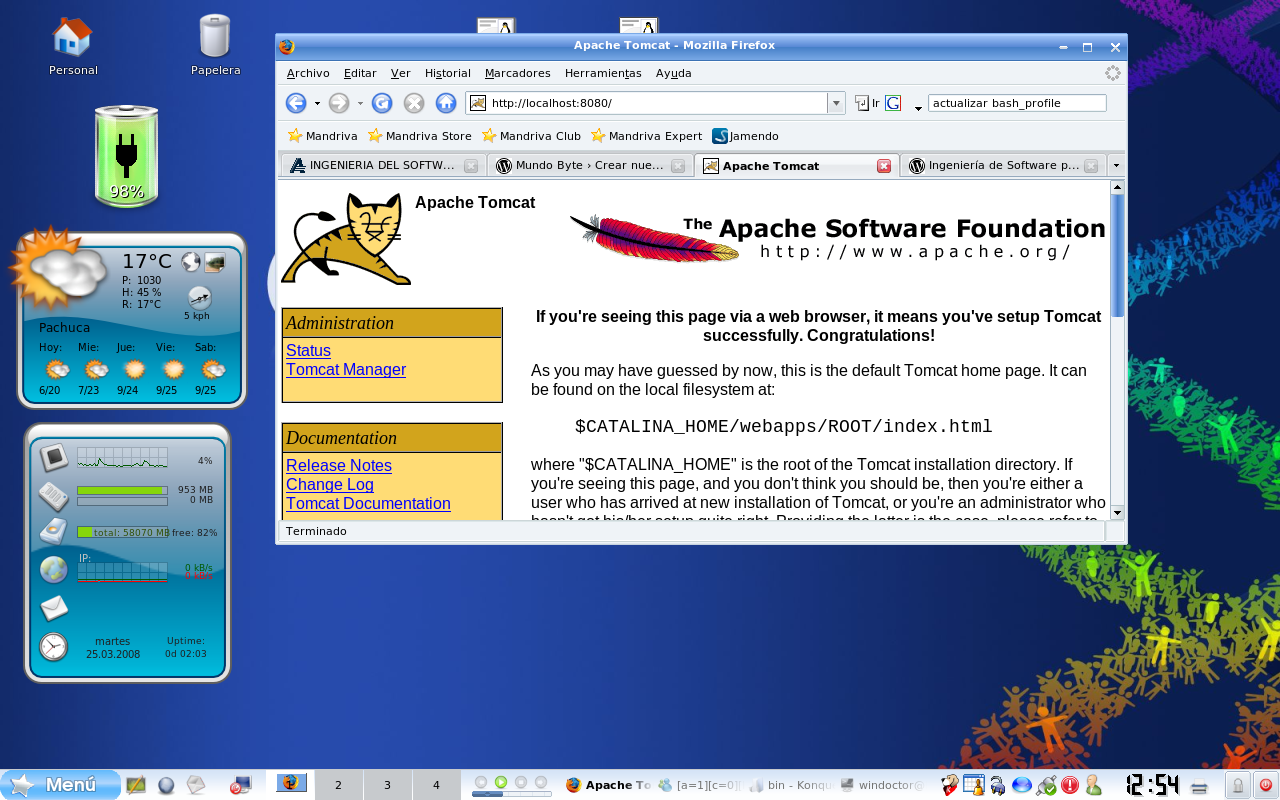
\includegraphics[height=0.20\textheight]{apache.png} \\
						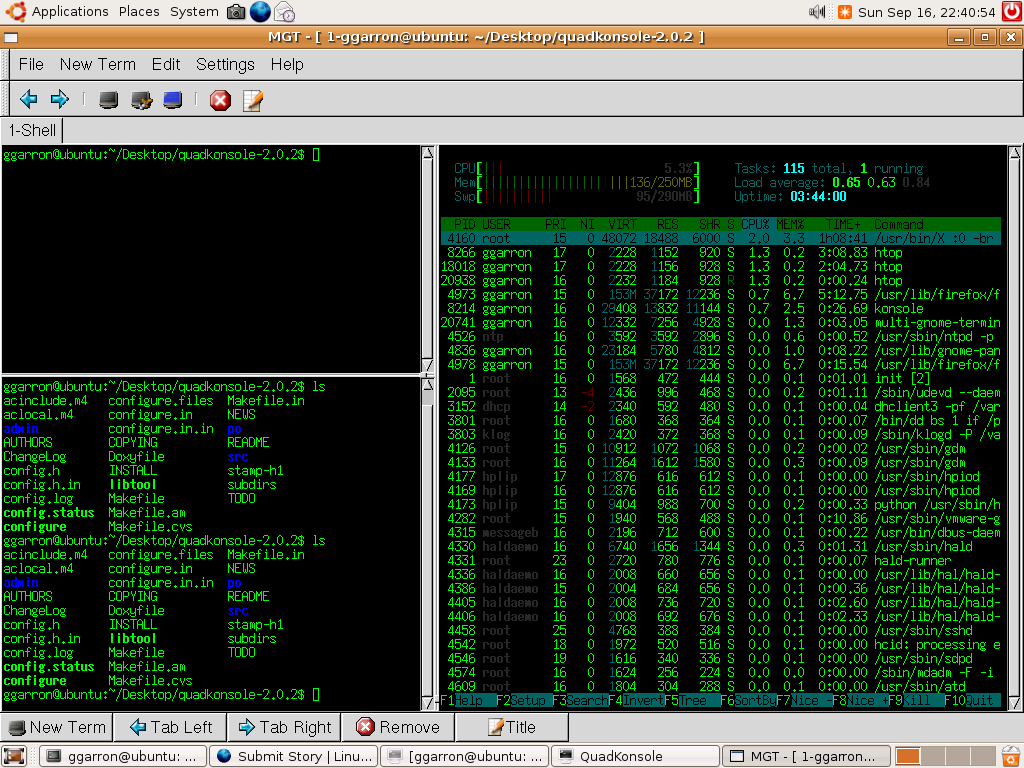
\includegraphics[height=0.20\textheight]{terminal.png}
					\end{center}
				
				\column{0.2\textwidth}{Cientifico}
					\begin{center}
						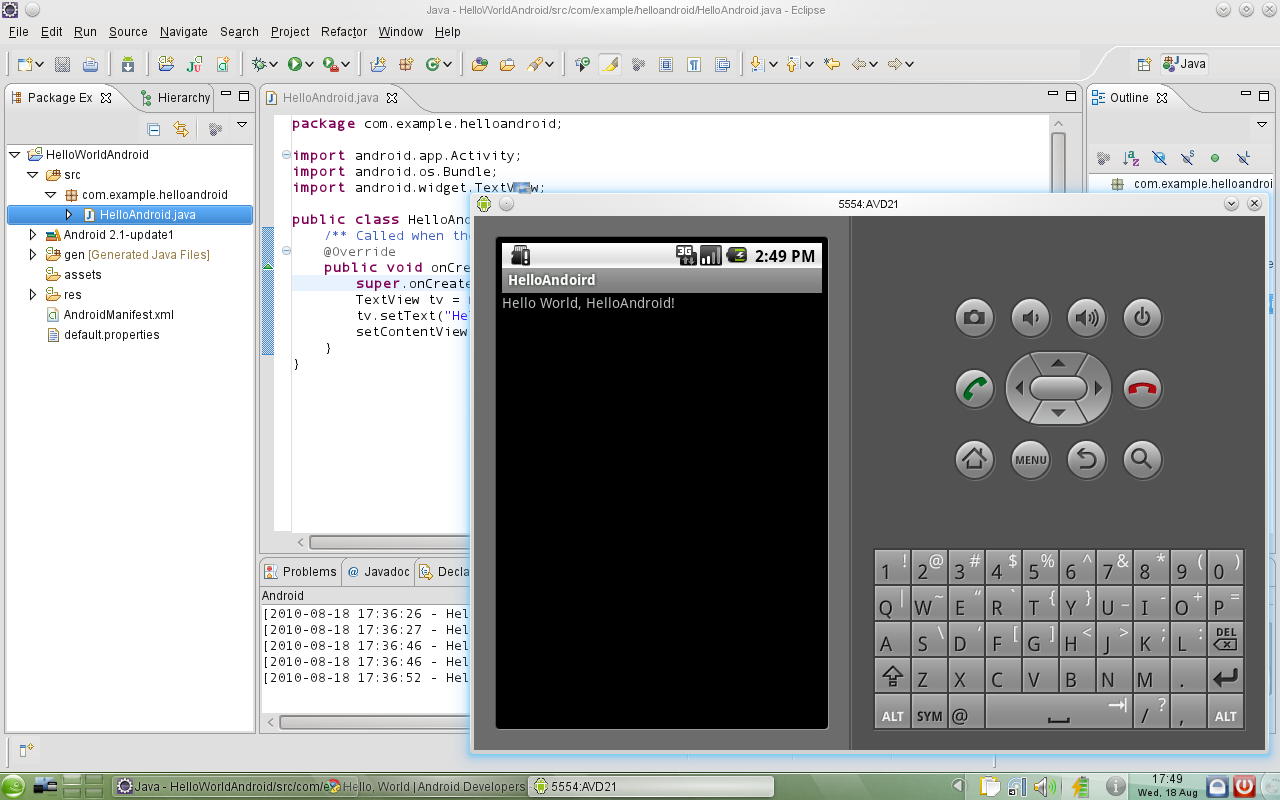
\includegraphics[height=0.20\textheight]{android.png} \\
						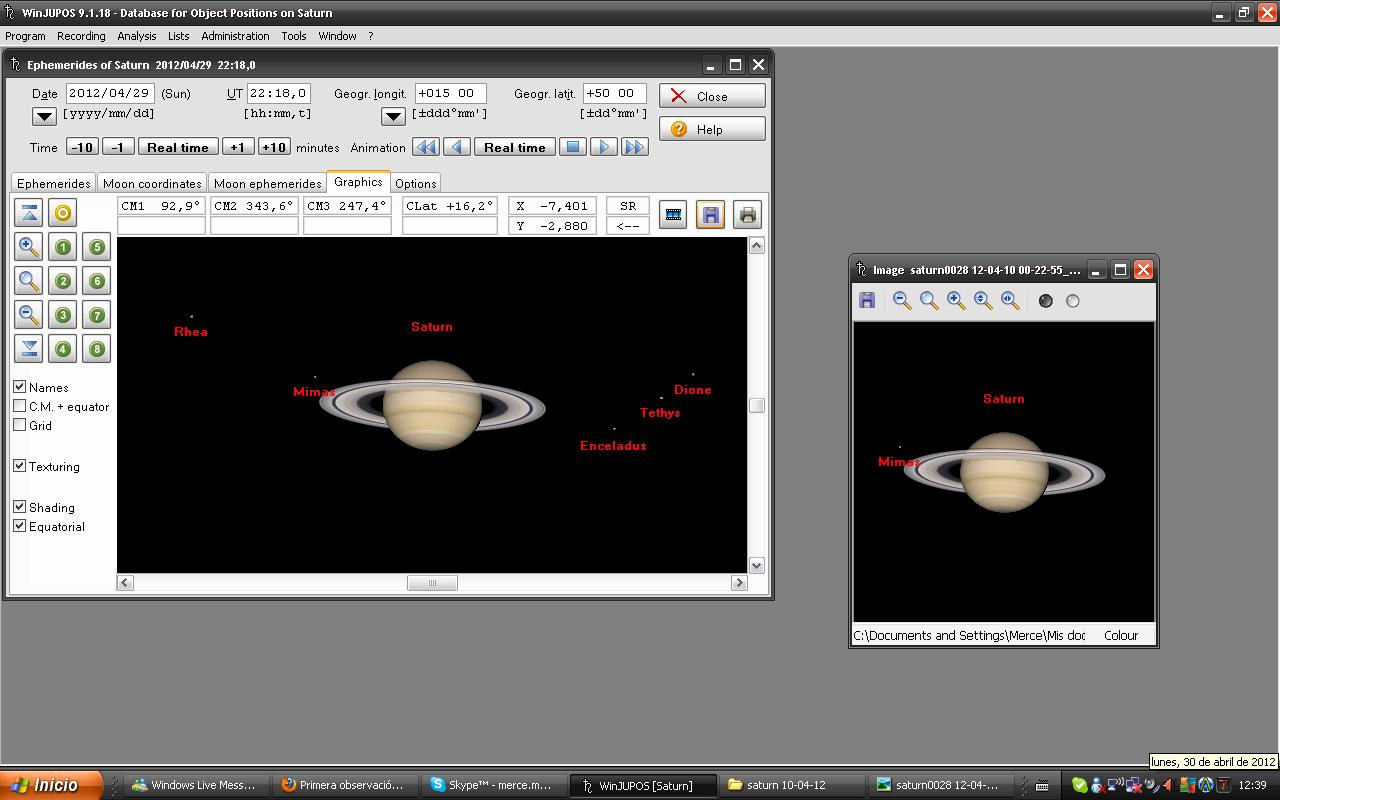
\includegraphics[height=0.20\textheight]{astro.jpg} \\
						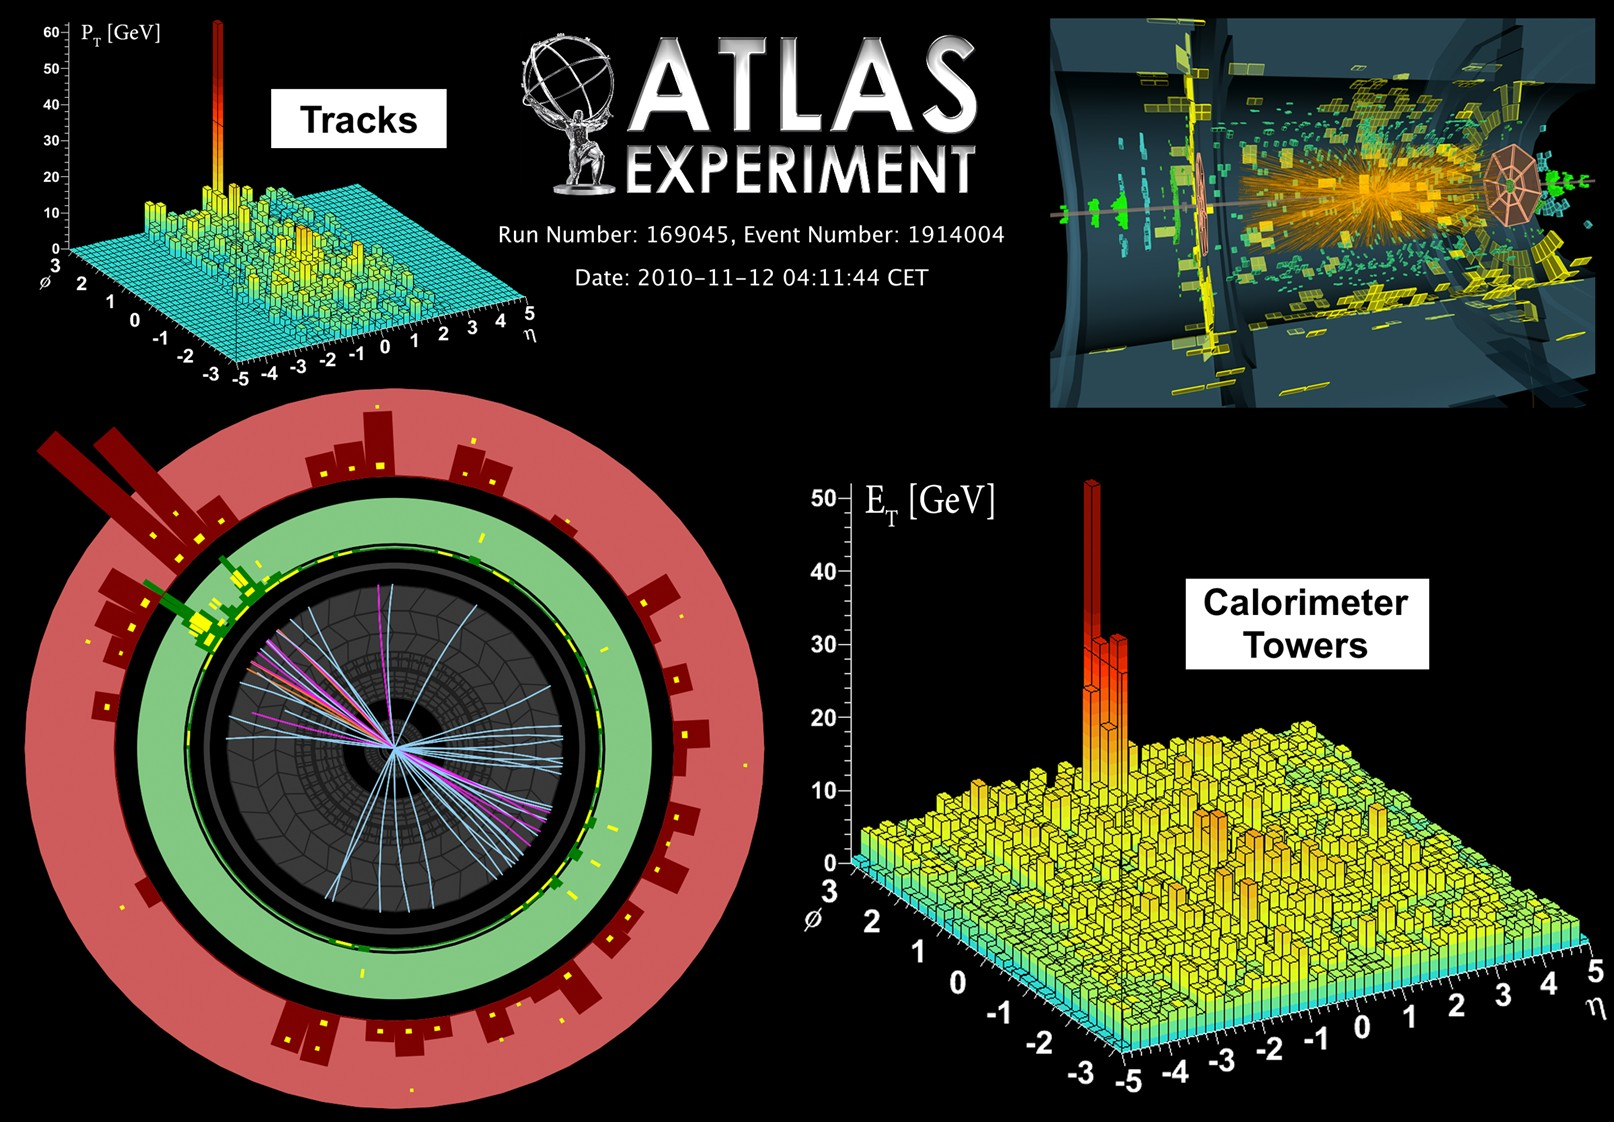
\includegraphics[height=0.20\textheight]{dpi.jpg}
					\end{center}
					
			\end{columns}
		
	\end{frame}

%%%%%%%%%%%%%%%%%%%%%%%%%%%%%% slide - 8.
%
%	\begin{frame}
%	
%		\frametitle{\textbf{Repositoio}}
%						
%			\begin{itemize}
%				\item Paqueteria
%				\item Software Disponible
%				\item Manejadores de paquetes
%			\end{itemize}
%
%	\end{frame}
%
%%%%%%%%%%%%%%%%%%%%%%%%%%%%%% slide - 9.

	\begin{frame}
	
		\frametitle{\textbf{Repositoio:}:[Software disponible]}
			
			\begin{itemize}{La cantidad de software disponible para Linux solo se limita dos cosas.}
				\item Existe?
				\item Es libre?
			\end{itemize}
			
			El ultimo conteo de software para distribuciones fue hace tanto que contabilizar la cantidad de aplicaciones disponibles para una sola distribucion es demaciado dificil. \\
			
			\begin{columns}
			
				\column{0.3\textwidth}{Debian}
					
\includegraphics[height=0.25\textheight]{debian.png}

				\column{0.3\textwidth}{Open Suse}
					
\includegraphics[height=0.25\textheight]{opensuse.png}
				
				\column{0.3\textwidth}{Fedora}
					
\includegraphics[height=0.25\textheight]{fedora.png}
					
			\end{columns} 
			
	\end{frame}

%%%%%%%%%%%%%%%%%%%%%%%%%%%%%% slide - 10.

	\begin{frame}
	
		\frametitle{\textbf{Repositoio:}:[Paqueteria]}
		
			Un paquete es un grupo de programas o librerias necesarios para hacer funcional al software que se desea instalar; algo muy similar a los exe de windows, solo que a diferencia de estos, no son ejecutables... 
			
			\begin{center}
				
\includegraphics[height=0.30\textheight]{app.jpg}
			\end{center}
			
			Existen tres tipo principales de paqueteria:
			
			\begin{columns}
			
				\column{0.2\textwidth}{DEB}
					
\includegraphics[height=0.20\textheight]{deb.png}

				\column{0.2\textwidth}{RPM}
					
\includegraphics[height=0.20\textheight]{rpm.png}
				
				\column{0.2\textwidth}{BINARIO}
					
\includegraphics[height=0.20\textheight]{bin.png}
					
			\end{columns} 
		
	\end{frame}
	
%%%%%%%%%%%%%%%%%%%%%%%%%%%%%% slide - 11.

	\begin{frame}
	
		\frametitle{\textbf{Repositoio:}:[Manejadores de Paquetes]}
		
			El manejador de paquetes es el encargado de gestionar la transaccion de paquetes entre nuestro PC y los servidores de aplicaciones. \\		
			El sistema de paquetes analiza esta informaci\'on para permitir la b\'usqueda de paquetes, actualizar las librer\'ias y aplicaciones instaladas, revisar que todas las dependencias se cumplan y obtenerlas si no se cuenta con ellas de manera autom\'atica.
			
			\begin{itemize}{Los manejadores de paquetes mas usados:}
				\item APT Manejador de Paquetes de Debian Linux
				\item YUM Manejador de Paquetes de Redhat Linux
				\item SLAPT Manejador de Paquetes de Slackware Linux
				\item EBUILDS Manejador de Paquetes de Gentoo Linux
				\item PACMAN Manejador de Paquetes de ArchLinux
				\item PET Manejador de Paquetes de Puppy Linux
			\end{itemize}

	\end{frame}

%%%%%%%%%%%%%%%%%%%%%%%%%%%%%% slide - 12.

	\begin{frame}
	
		\frametitle{\textbf{Repositoio:}:[...Manejadores de Paquetes]}
		
			Existe tambien otros tipos de paqueterias:
			
			\begin{columns}
			
				\column{0.2\textwidth}{PKG}
					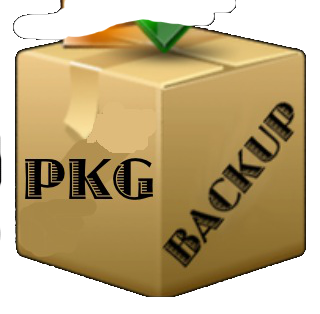
\includegraphics[height=0.20\textheight]{pkg.png}

				\column{0.2\textwidth}{TAR.GZ}
					
\includegraphics[height=0.20\textheight]{targz.png}
				
				\column{0.2\textwidth}{X}
					
\includegraphics[height=0.20\textheight]{xz.png}
					
			\end{columns} 
		
			Tambien existen otras formas de instalacion de software:
			
			\begin{columns}
			
				\column{0.2\textwidth}{Ejecutando Scripts}
					
\includegraphics[height=0.20\textheight]{bash.png} \\
					(*.sh, *.py, *.ruby, *.perl)

				\column{0.2\textwidth}{Compilando Codigo}
					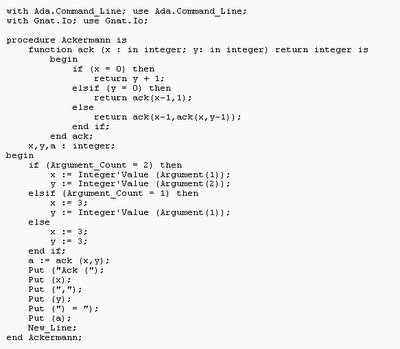
\includegraphics[height=0.20\textheight]{source.png} \\
					(C, C++, Java, C#)
				
				\column{0.2\textwidth}{Emulando Windows}
					
\includegraphics[height=0.20\textheight]{wine.png} \\
					(Crossover, DosBox, PlayOnLinux)
					
			\end{columns}

	\end{frame}
	
%%%%%%%%%%%%%%%%%%%%%%%%%%%%%% slide - 13.
%
%	\begin{frame}
%	
%		\frametitle{\textbf{Configuracion}}
%						
%			\begin{itemize}
%				\item Donde encontar Linux?
%				\item Que necesito para usar Linux?
%				\item Donde puedo consegir ayuda?
%			\end{itemize}
%
%	\end{frame}
%
%%%%%%%%%%%%%%%%%%%%%%%%%%%%%% slide - 14.

	\begin{frame}
				
		\begin{block}{\textbf{Configuracion:}:[Donde encontrar linux?]}
						
			Linux es de libre descarga en Internet y se puede encontrar instalado casi en cualquier dispocitivo.
			
			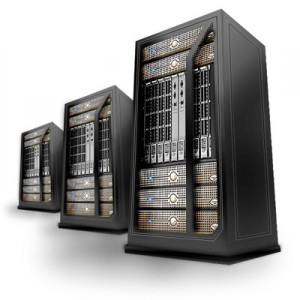
\includegraphics[height=0.20\textheight]{server.png}
			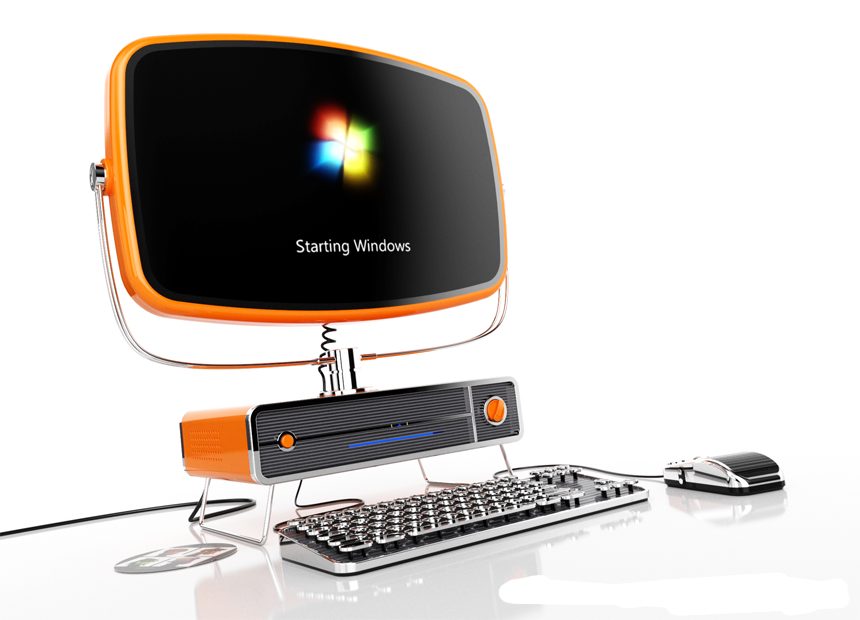
\includegraphics[height=0.20\textheight]{pc.png}
			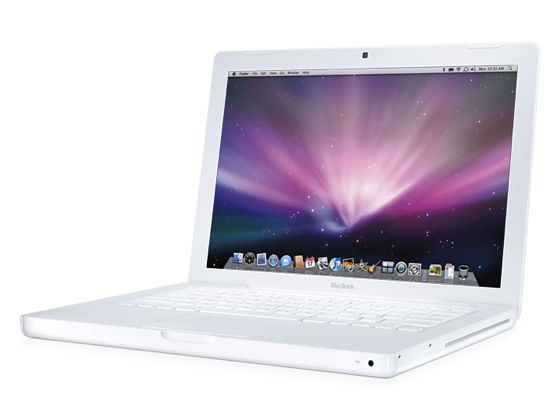
\includegraphics[height=0.20\textheight]{laptop.png}
			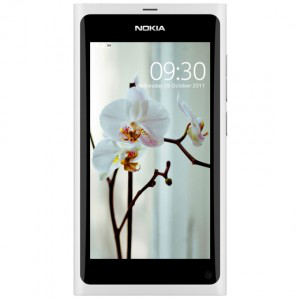
\includegraphics[height=0.20\textheight]{cell.png}
			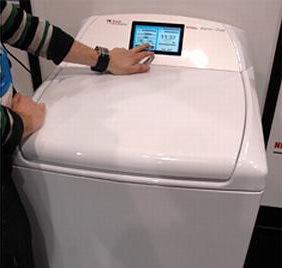
\includegraphics[height=0.20\textheight]{electro.png}
			
		\end{block}
	
		\begin{block}{\textbf{Configuracion:}:[Que necesito para usar Linux?]}
						
			Linux es de libre descarga en Internet y se puede encontrar instalado casi en cualquier dispocitivo.
			
			
\includegraphics[height=0.20\textheight]{linux-logo.png}
			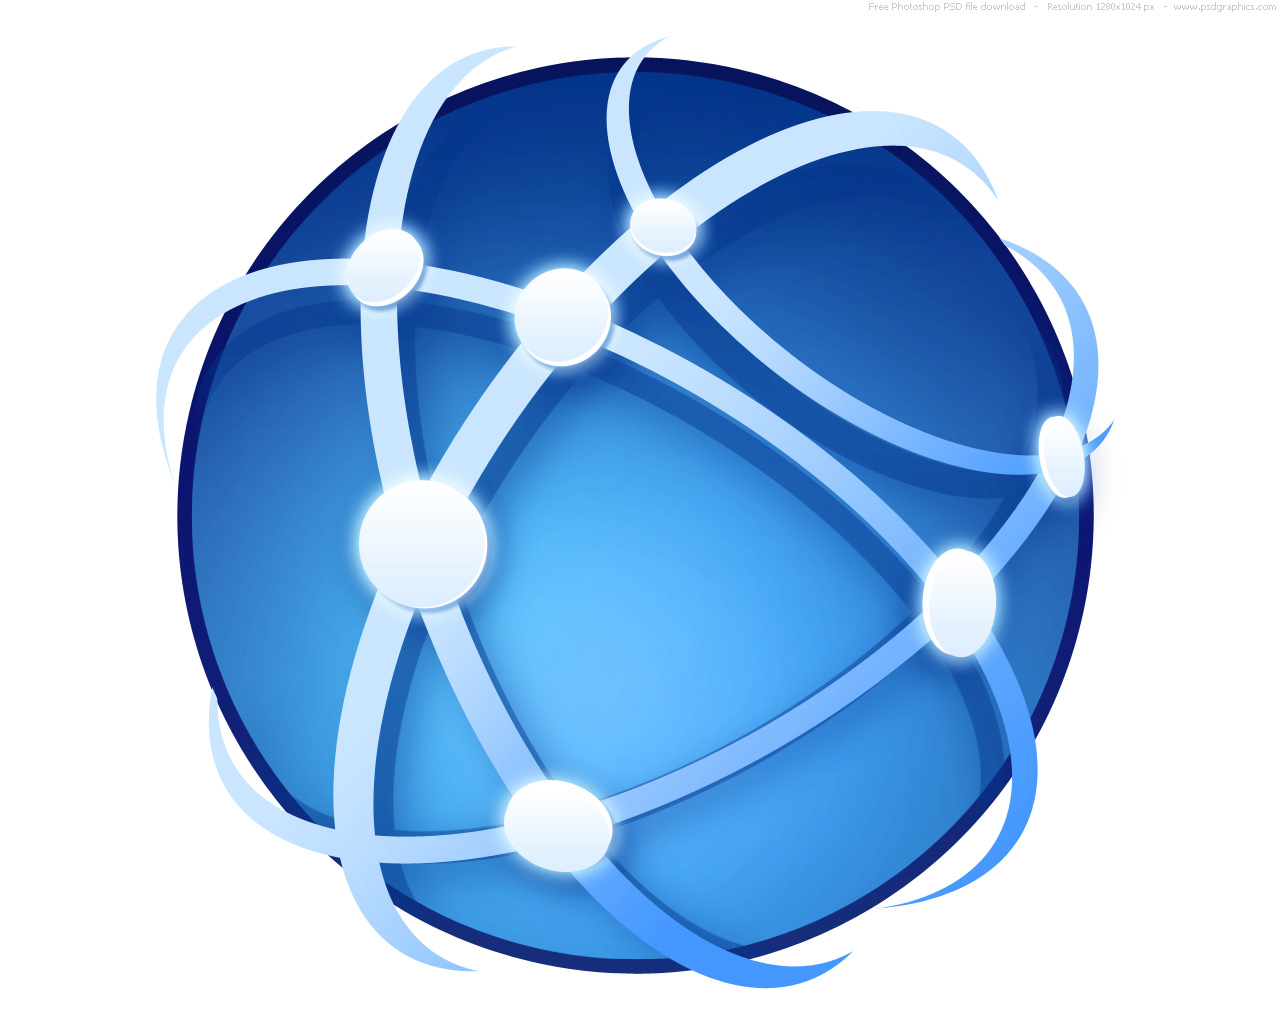
\includegraphics[height=0.20\textheight]{internet.png}
		
		\end{block}
			
		\begin{block}{\textbf{Configuracion:}:[Donde puedo consegir ayuda?]}
			
			http://linuxtour.org/Listas  \\
			comunidadlinuxuni@gmail.com
			
		\end{block}
			
	\end{frame}
	
\end{document}
	
